% !TeX root = main.tex

\documentclass{beamer}

\usepackage{pgfplots}
\usepackage{graphicx}
\usepackage{caption}
\usepackage{ragged2e}
\usepackage{setspace}
\usepackage{comment}
\usepackage{csquotes}
\usepackage{float}
\usepackage{svg}
\usepackage{multicol}\columnseprule 0.4pt\raggedcolumns
\usepackage[utf8]{inputenc}
\usepackage{hyperref}

\usepackage{siunitx}
\sisetup{%quotient-mode=fraction,
		output-decimal-marker = {.},
		per-mode = fraction,
		separate-uncertainty = true,
		multi-part-units=single,
		exponent-product = \cdot,
		range-phrase=--}

\setbeamertemplate{footline}[frame number]

\setbeamertemplate{footline}{%
  \leavevmode%
  \hbox{\begin{beamercolorbox}[wd=0.565\paperwidth,ht=0ex,dp=0ex,right]{frame number}%
    \vskip0pt
    \usebeamerfont{footline}\usebeamercolor[fg]{footline}
    \insertframenumber/\inserttotalframenumber
    \vskip0.5ex
    \end{beamercolorbox}%
  }%
  \vskip0pt%
}

\usetheme{Hannover}
\usecolortheme{orchid}
\definecolor{sidebar}{RGB}{34,34,138}
\setbeamercolor{sidebar}{bg=sidebar}
\setbeamercolor{title in sidebar}{fg=white}
\setbeamercolor{author in sidebar}{fg=white}
\setbeamercolor{section in sidebar}{fg=white}
\hypersetup{pdfpagemode=FullScreen}
\title{Capture the Flag Platform}
\subtitle{Made for UCloud, Adapted to GCP\\ \vspace{17pt} \includesvg[width=.3\textwidth]{images/SDU.svg}\vspace{-10pt}}
\author[K. B. Larsen]{Kian Banke Larsen}
\institute{Southern University of Denmark}
\date{\today}

\beamertemplatenavigationsymbolsempty

\begin{document}
\begin{frame}
\titlepage
\end{frame}

\section*{Outline}
\begin{frame}{Outline}
\tableofcontents
\end{frame}

\section{Introduction}
\begin{frame}{Introduction}
    \begin{itemize}
        \item What are we solving?
        \item Who are we solving it for?
        \item Why are why solving it?
        \item How are we solving it?
    \end{itemize}
\vspace*{\fill}
    \only<2>{
        \begin{center}
            Let us have a peek before we continue\ldots
        \end{center}
    }
\end{frame}

\section{Architecture}
\begin{frame}{Hybrid Architecture}
    \begin{figure}
        \centering
        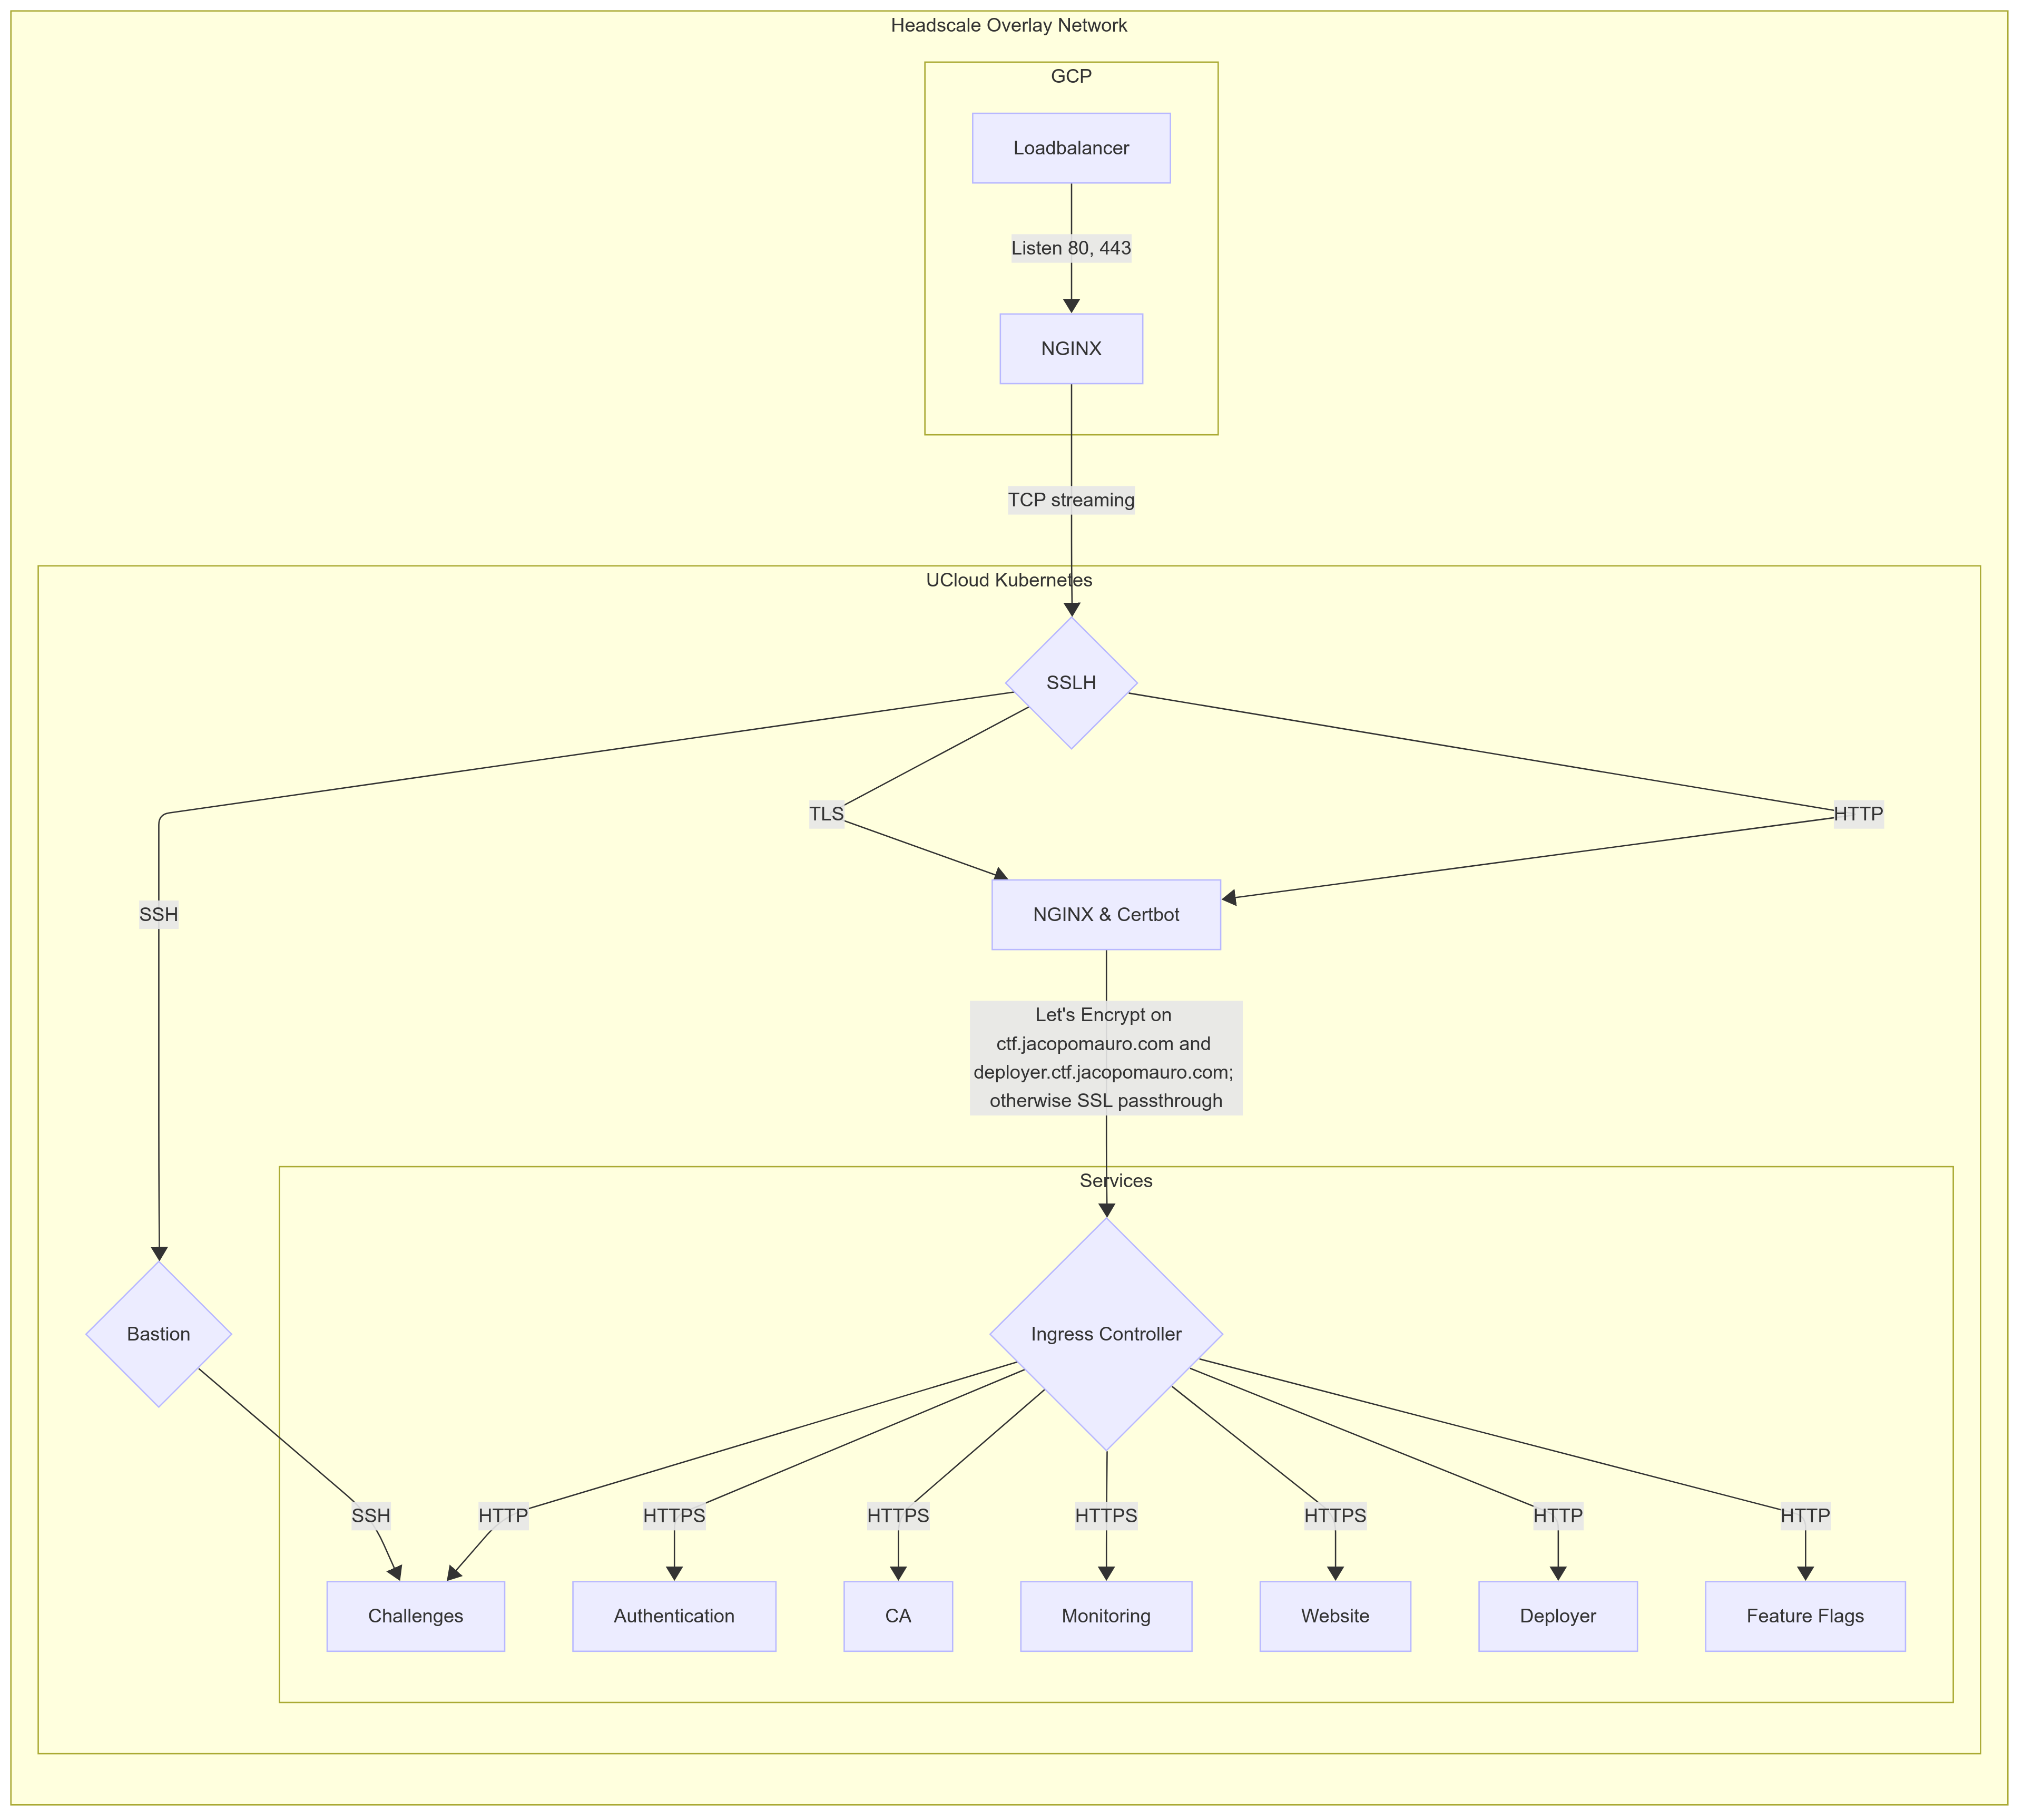
\includegraphics[width=.7\textwidth]{../report/images/ucloud-architecture.png}
        \caption{Architecture of the CTF platform deployed on UCloud/GCP.}
    \end{figure}
\end{frame}

\begin{frame}{GCP Architecture}
    \begin{figure}
        \centering
        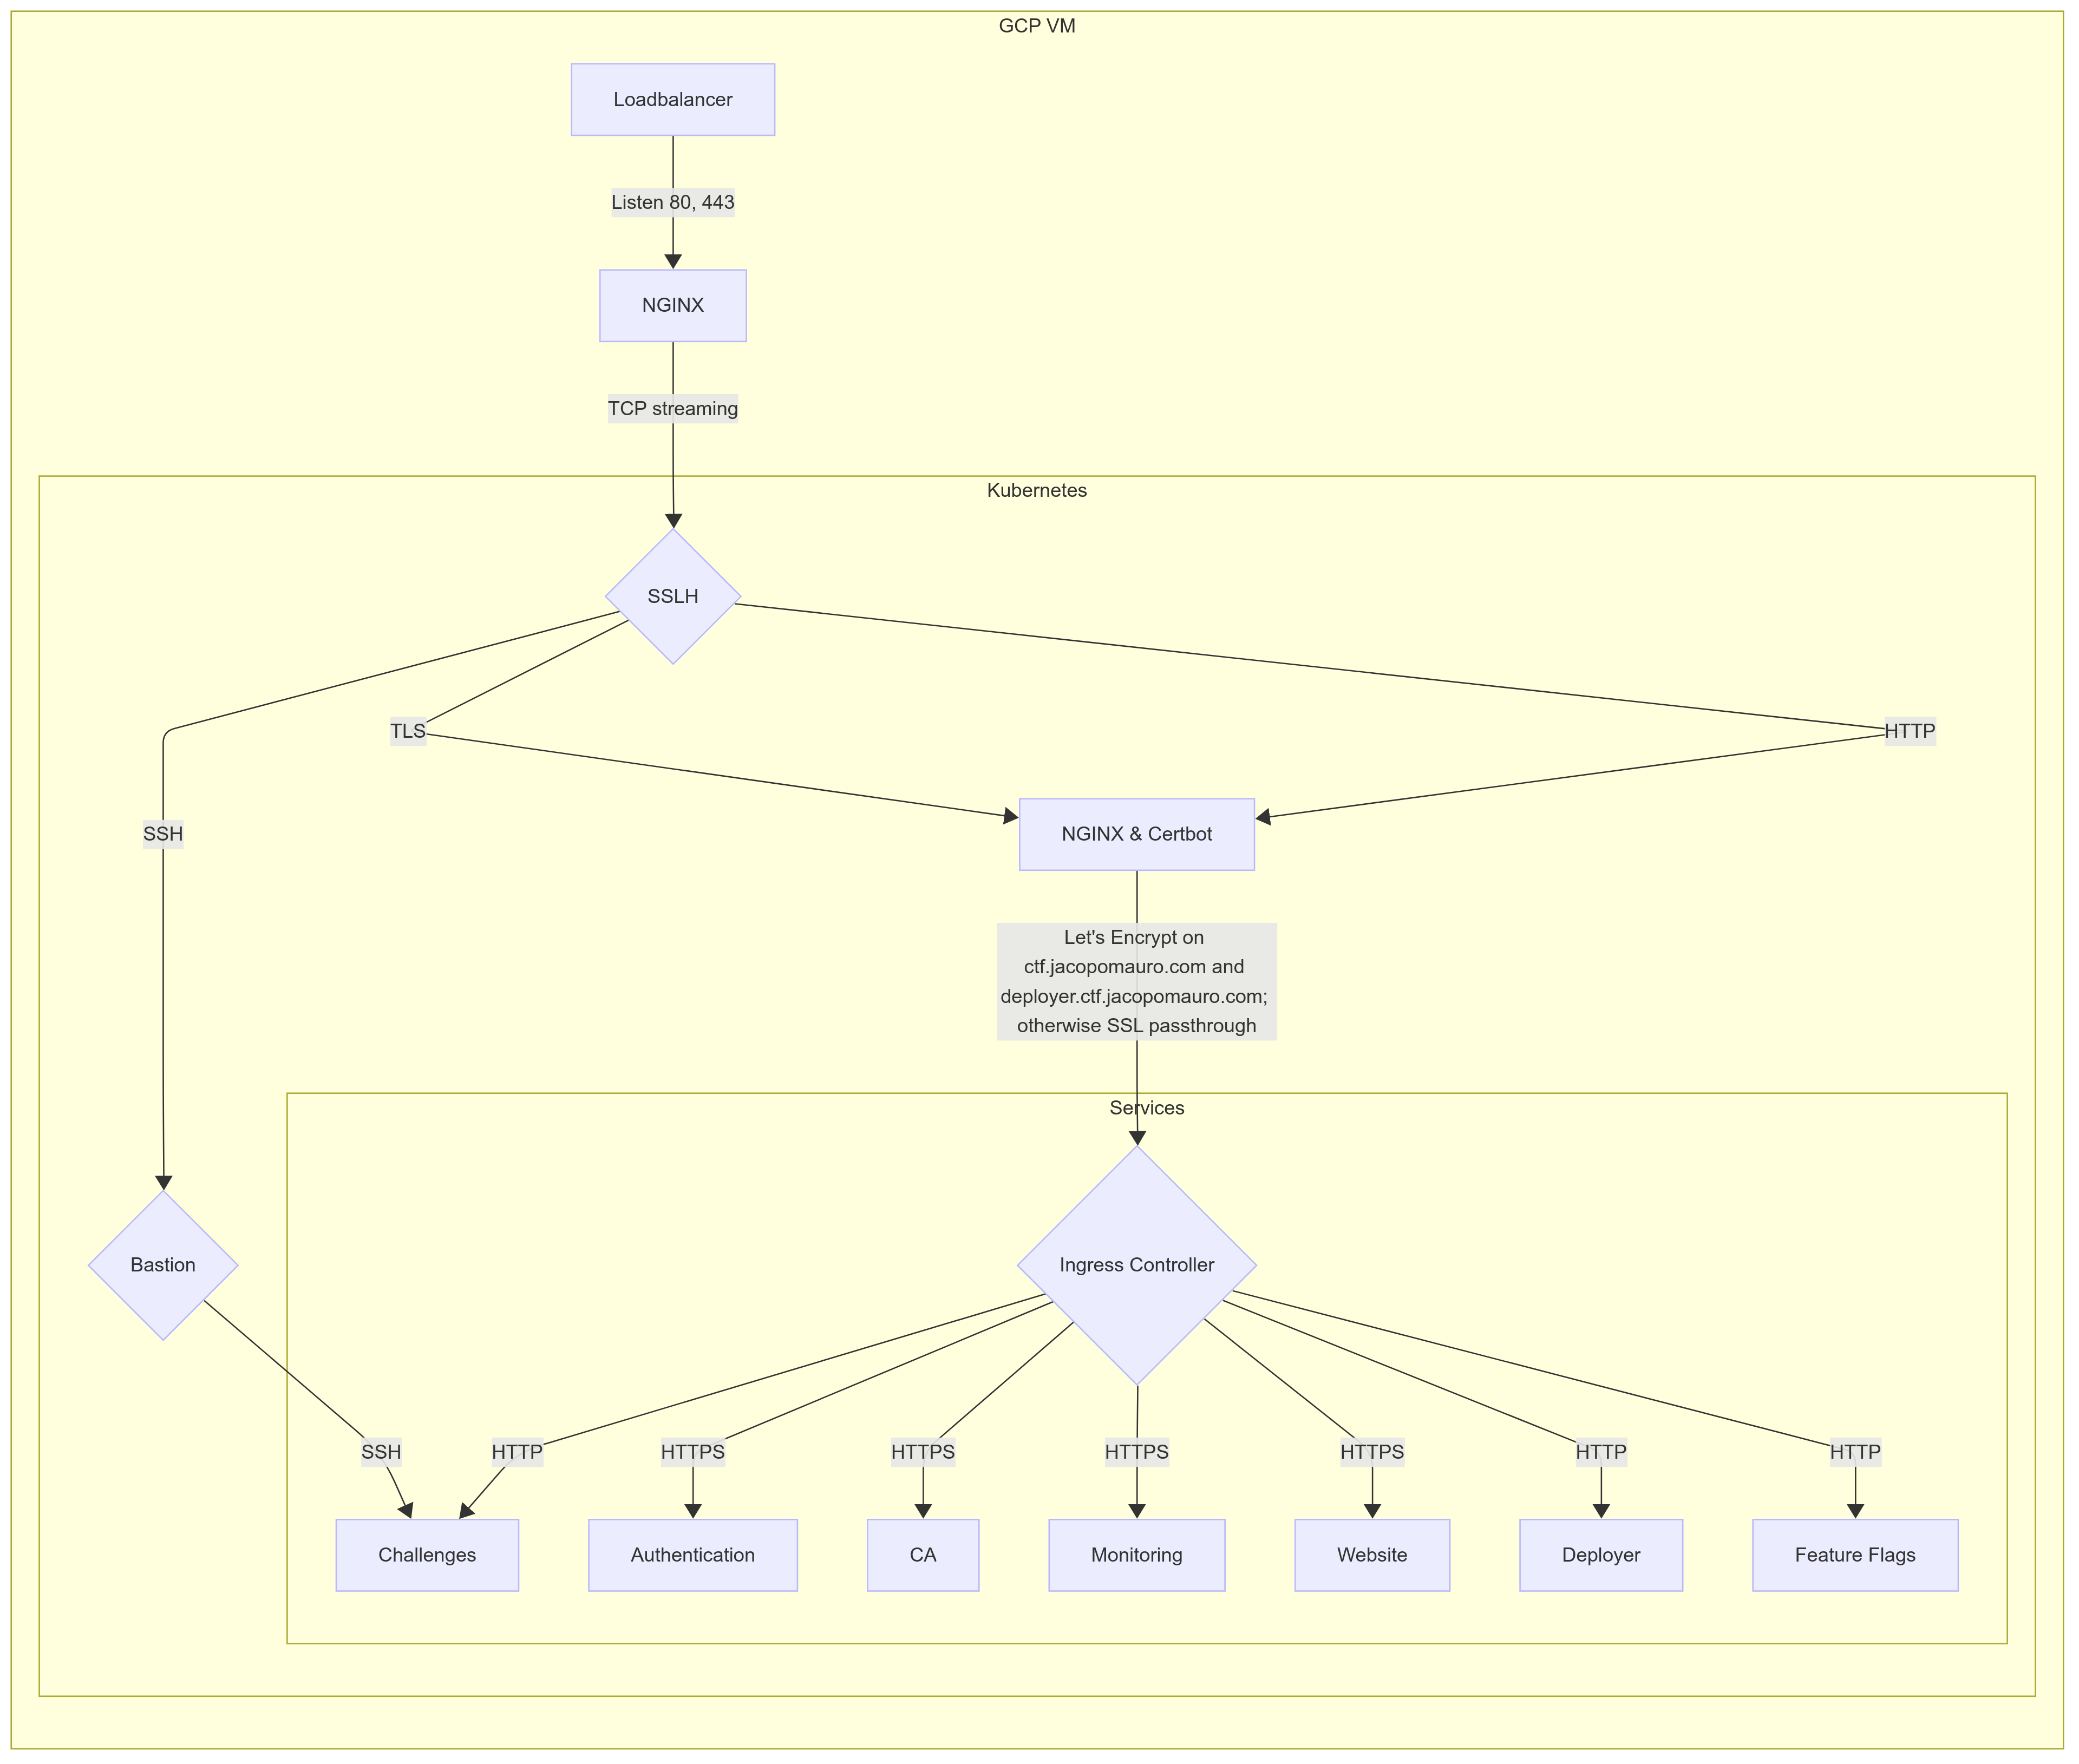
\includegraphics[width=.7\textwidth]{./images/GCP-architecture.png}
        \caption{Architecture of the CTF platform deployed on GCP.}
    \end{figure}
\end{frame}

\begin{frame}{UCloud Architecture}
    \only<1>{
    \begin{figure}
        \centering
        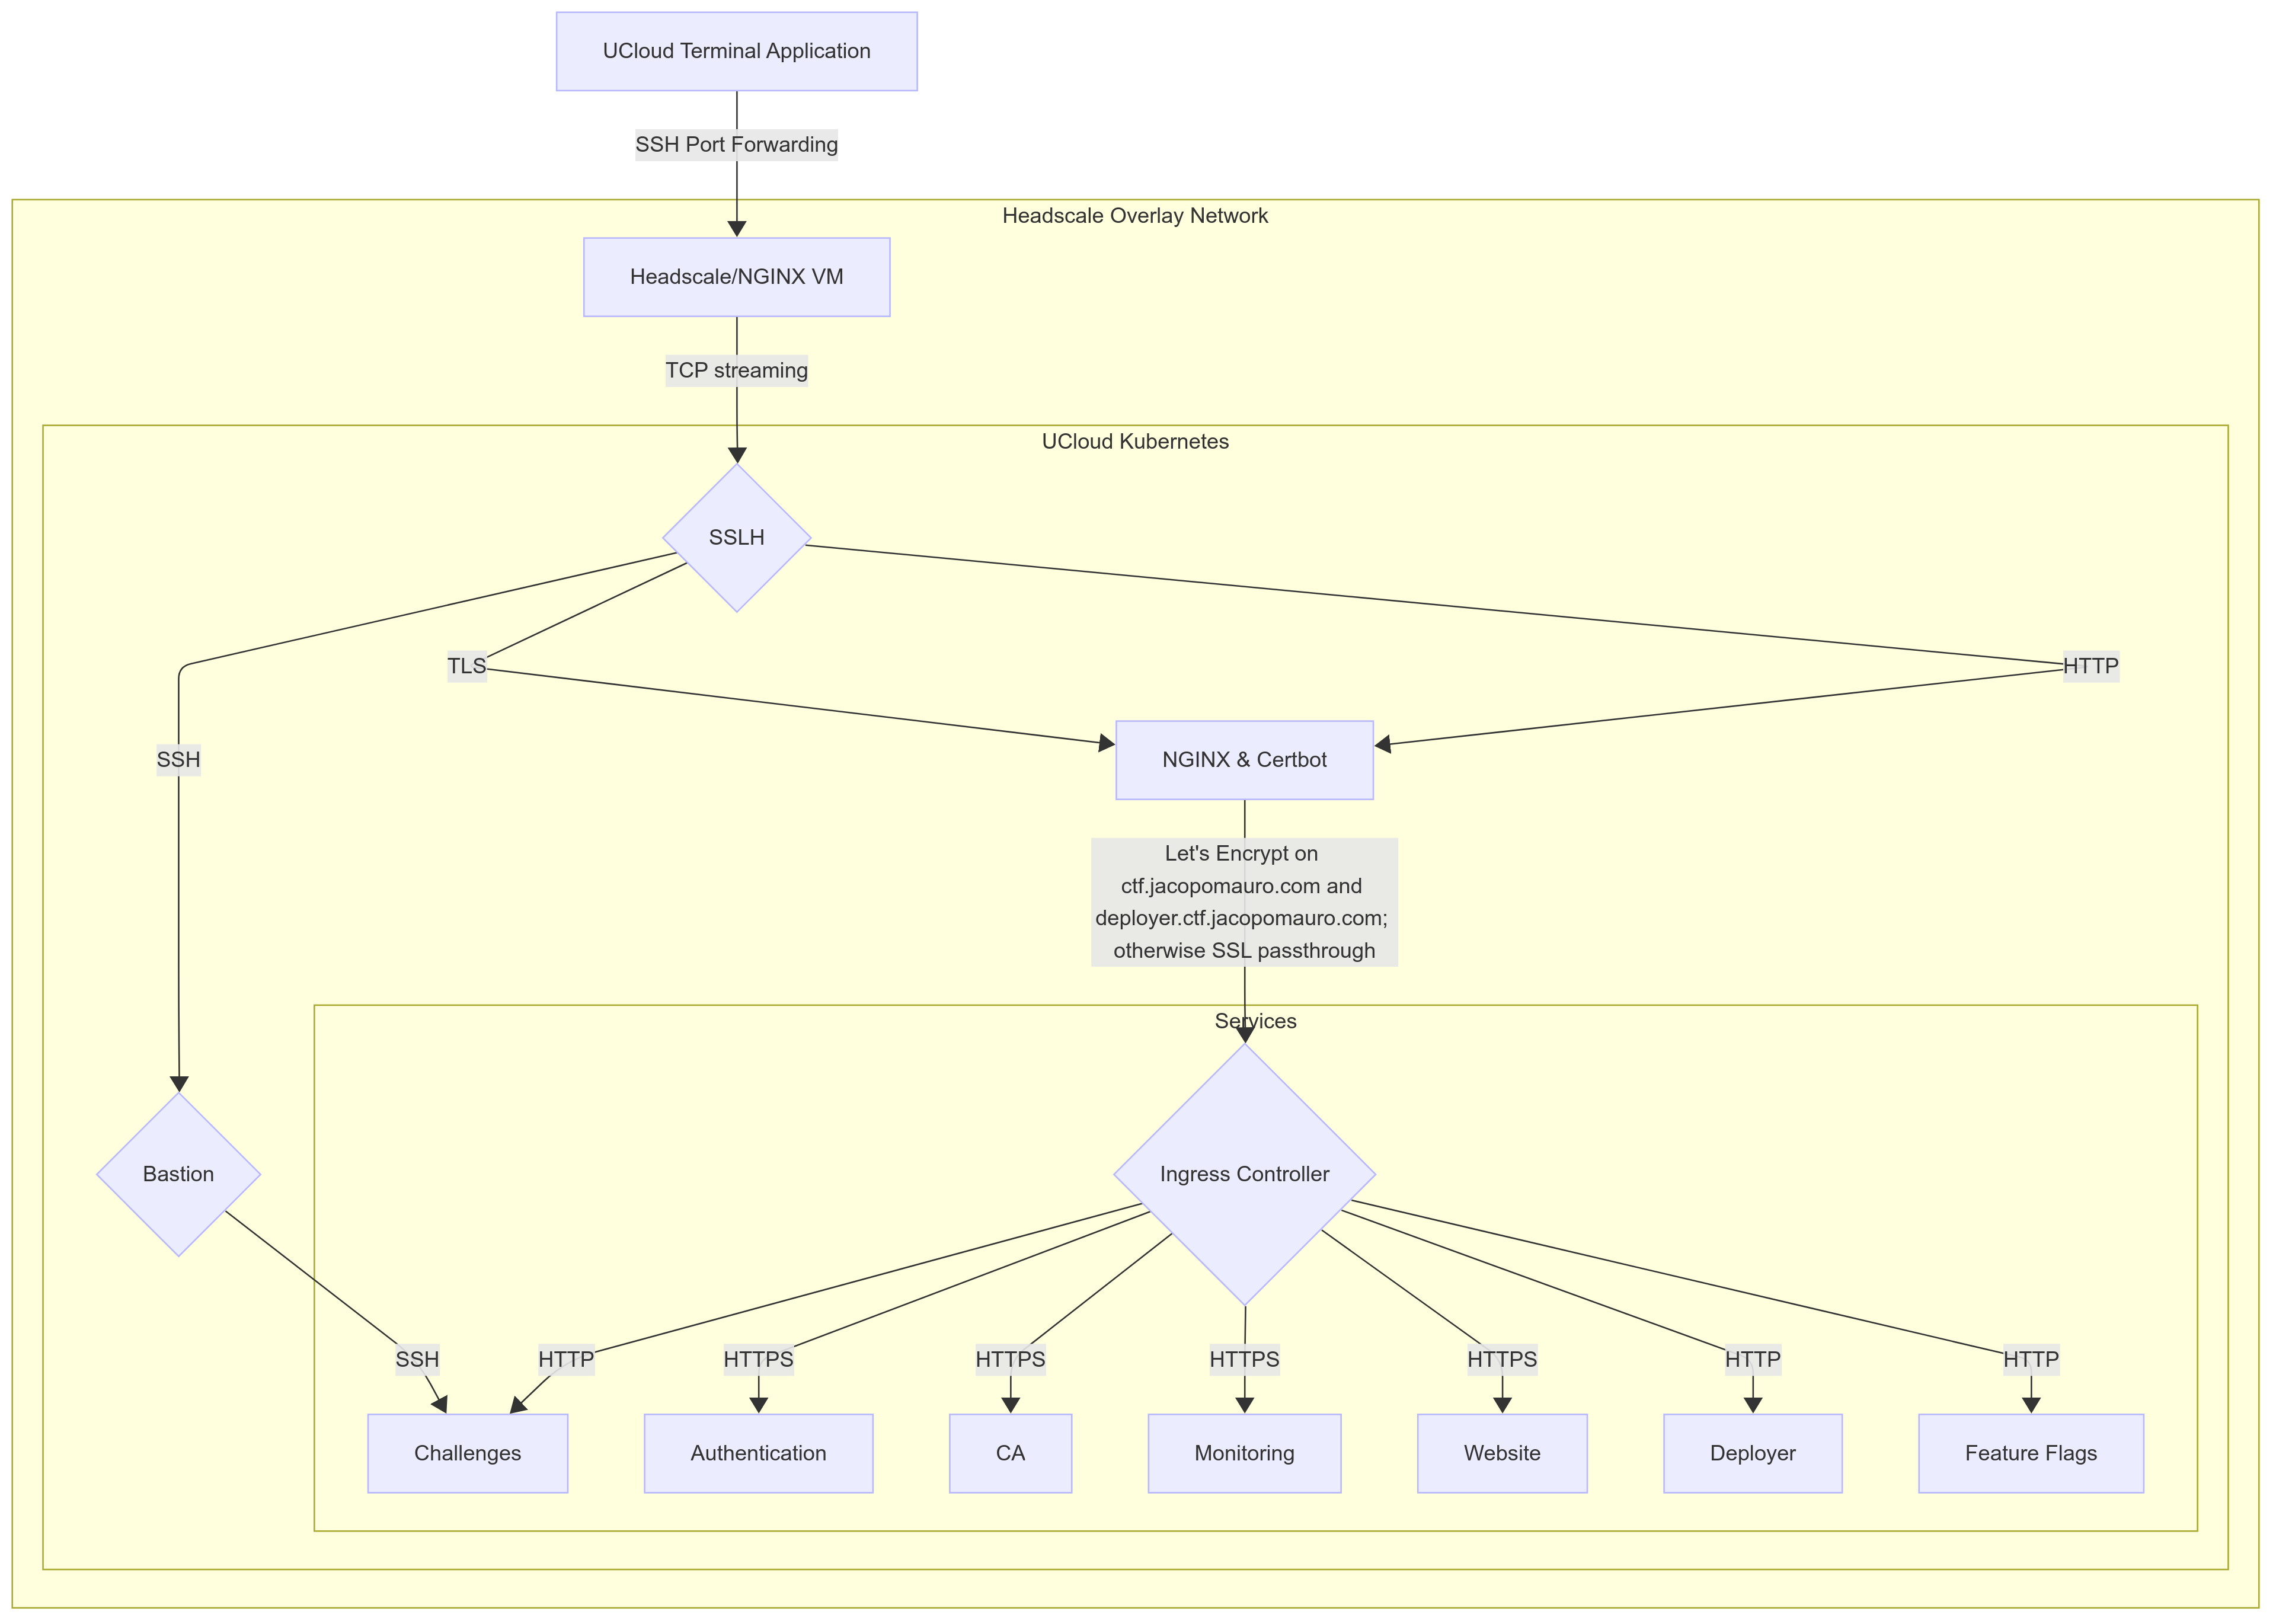
\includegraphics[width=.7\textwidth]{./images/UCloud-architecture.png}
        \caption{Architecture of the CTF platform deployed on UCloud. Not successfully implemented but possibly feasible.}
    \end{figure}
    }
    \only<2>{
    \begin{itemize}
        \item Connect to job functionality is not working.
        \item Cannot run Headscale on Docker service (NGNIX and Terminal).
        \item Only one public IP address per project.
        \item Managed to route traffic from terminal to VM using SSH port forwarding -- health endpoints responded. 
    \end{itemize}
    }
\end{frame}

\section{Storage}
\begin{frame}{Storage}
    \begin{figure}
        \centering
        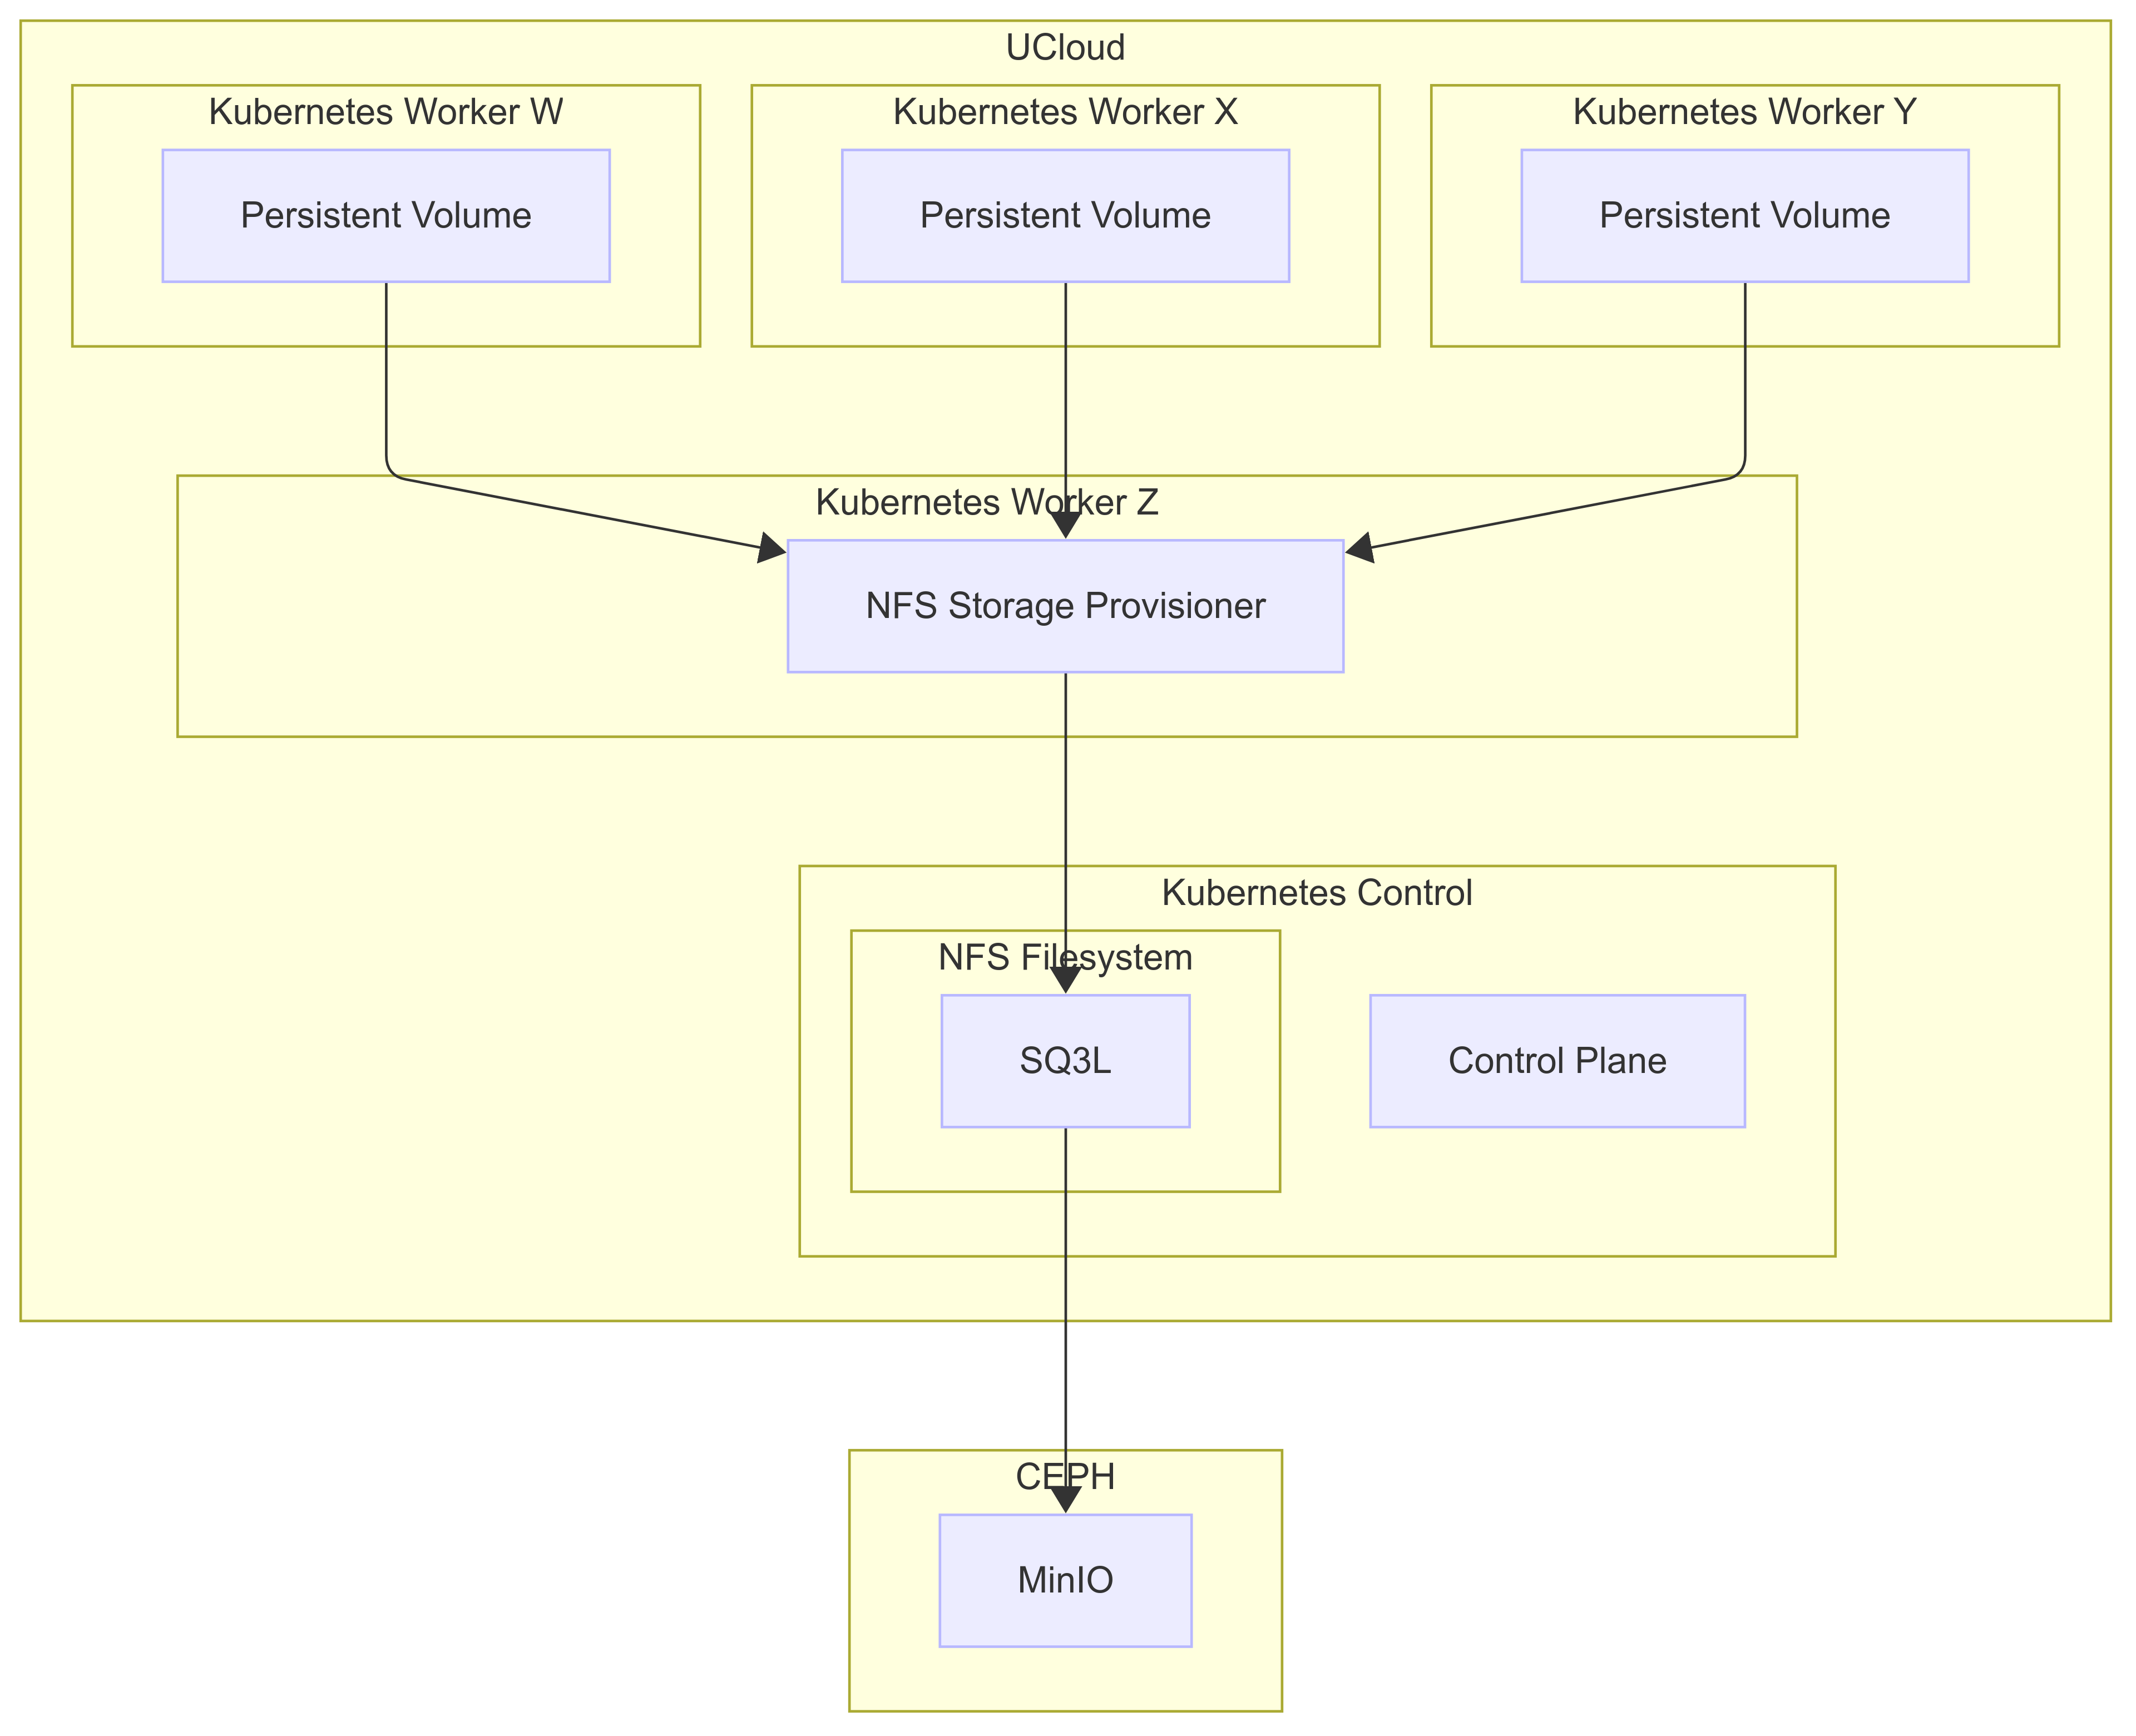
\includegraphics[width=.8\textwidth]{../report/images/storage-provisioner.png}
        \caption{Storage provisioning architecture of the CTF platform on UCloud using MinIO.}
    \end{figure}
\end{frame}

\section{Pulumi}
\begin{frame}{Stacks}
    \begin{figure}
        \centering
        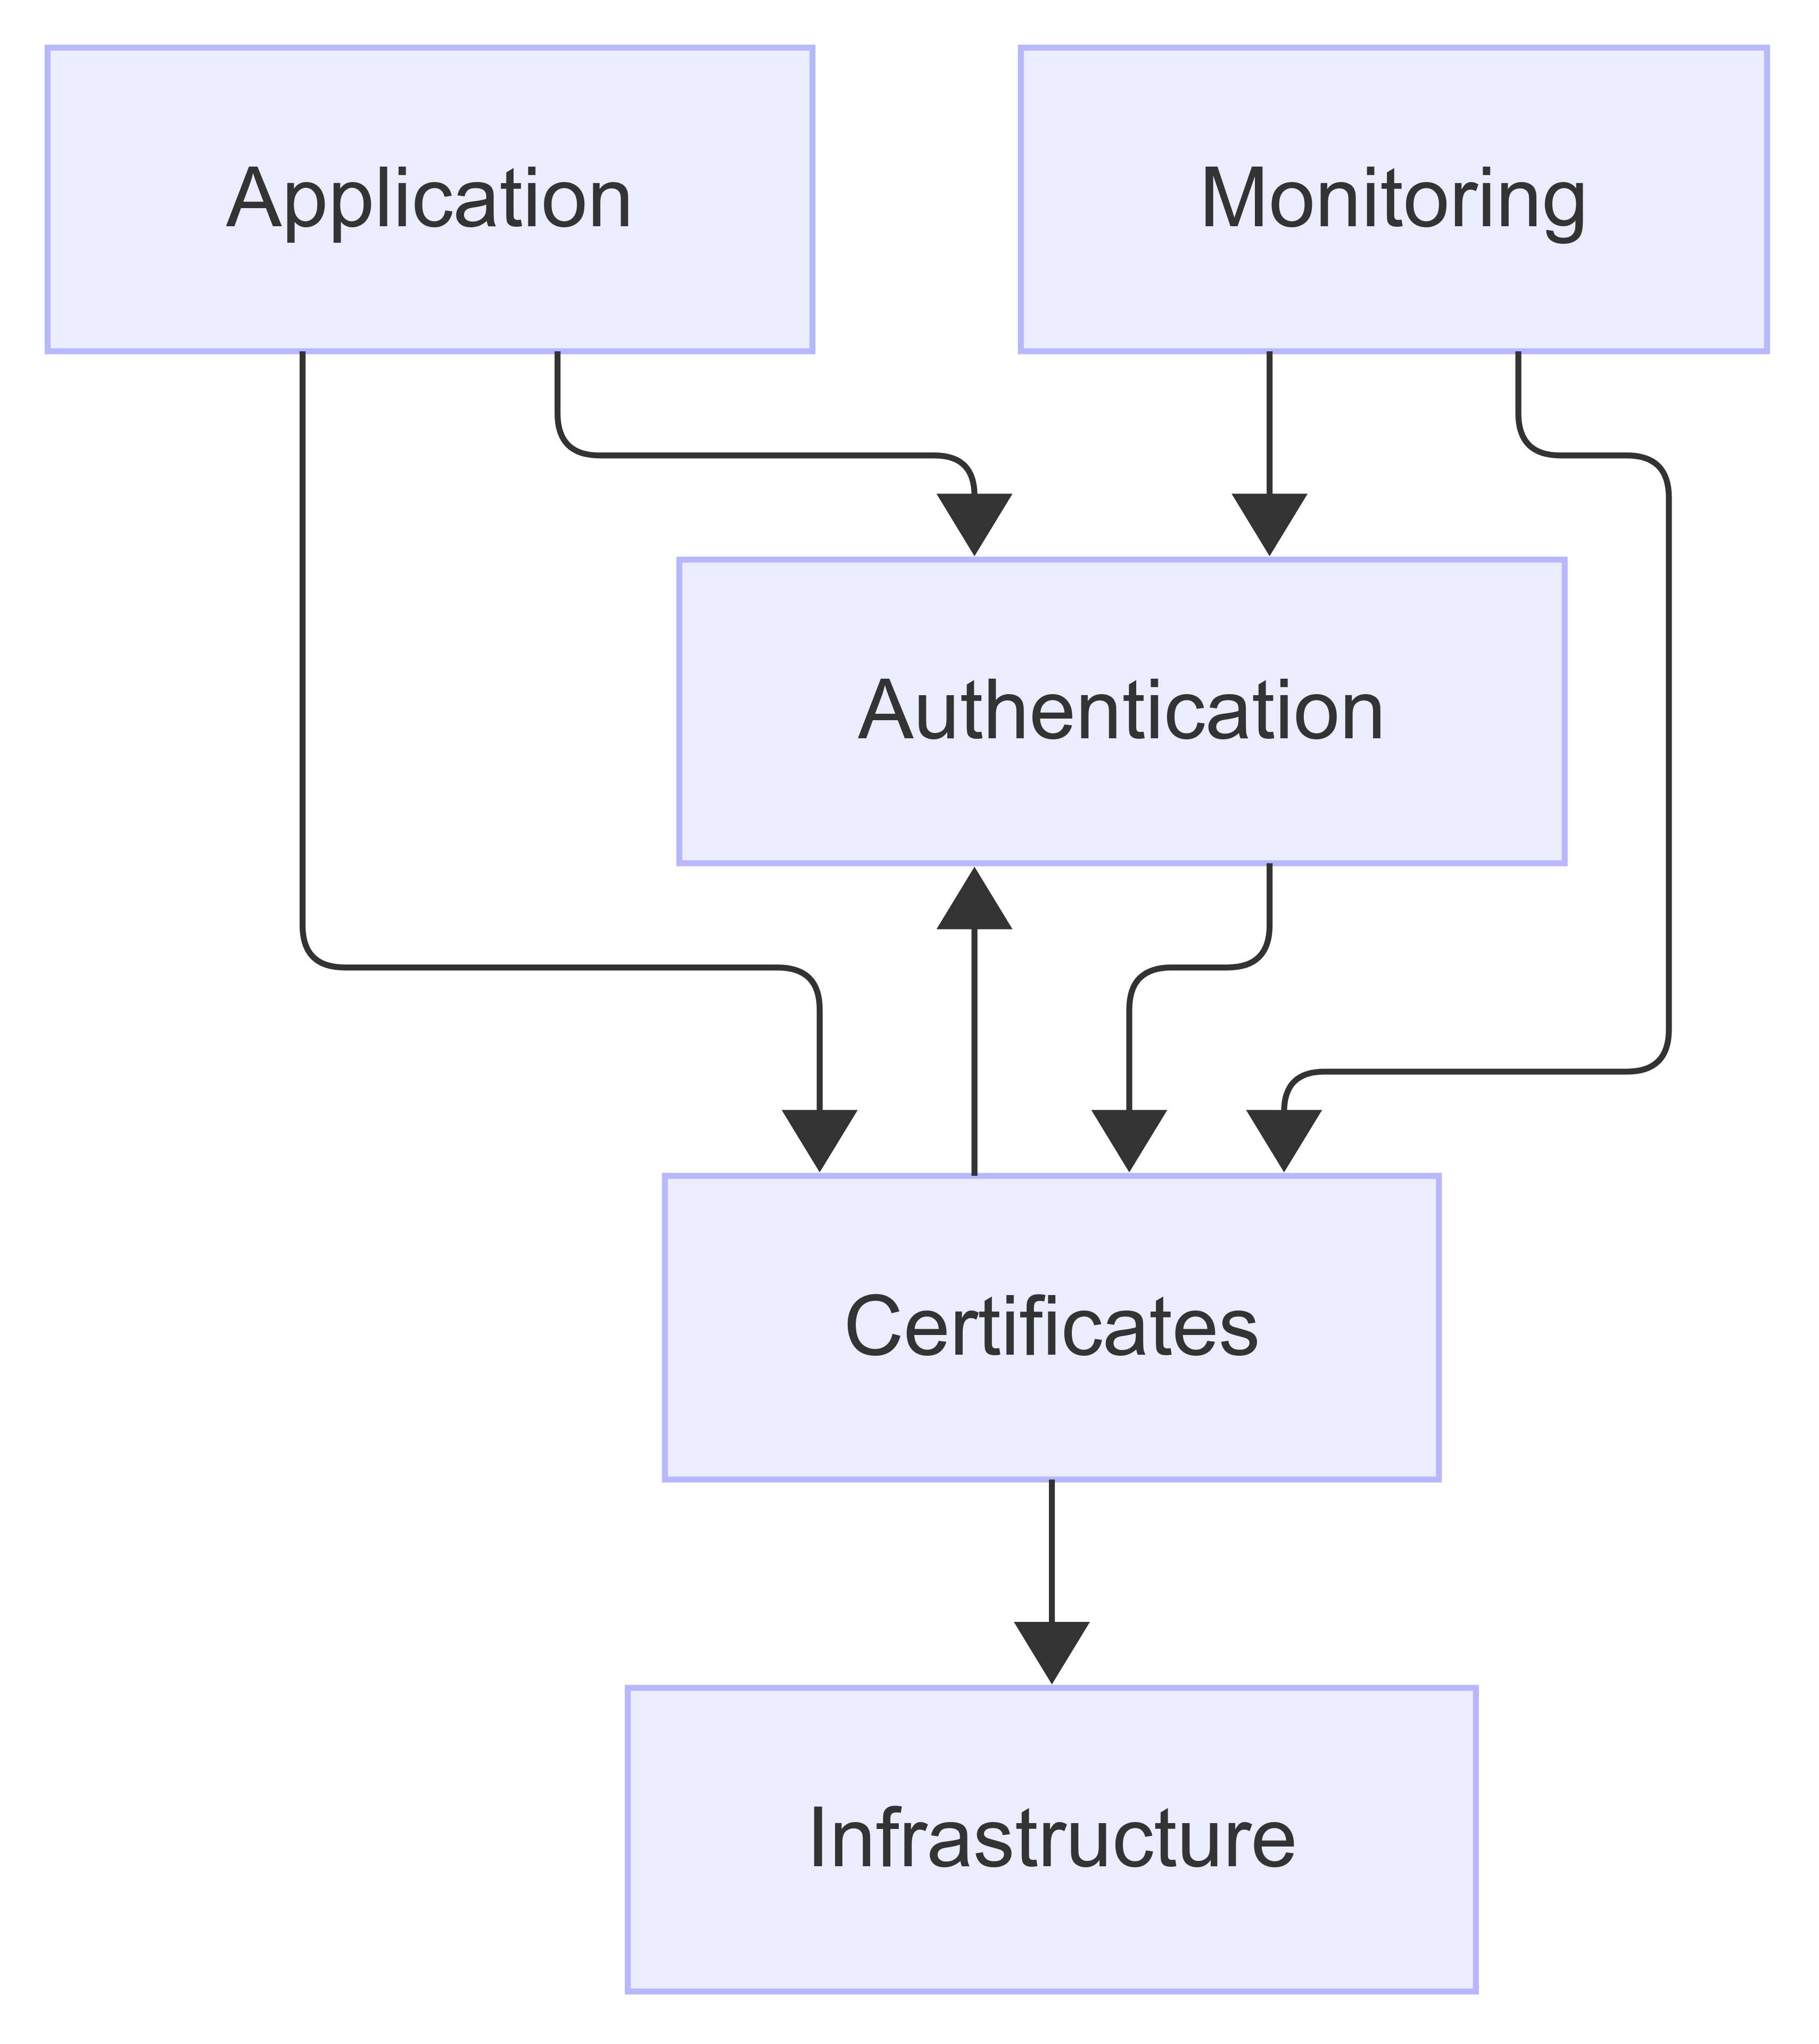
\includegraphics[width=.45\textwidth]{./images/pulumi-stacks.png}
        \caption{Pulumi Stacks Relationship. An arrow pointing from a source to a target indicates that the source depends on the target. Given the layered approach, these relationships are transitive.}
    \end{figure}
\end{frame}

\section{VMs}
\begin{frame}{Virtual Machines}
\begin{table}[h]
\centering
\begin{tabular}{|l|l|l|l|l|}
\hline
\textbf{Test Run} & \textbf{PC HV} & \textbf{GCP HV} & \textbf{PC HE} & \textbf{PC Containers} \\ \hline
1 & \SI{100}{\second} & \SI{123}{\second} & \SI{420}{\second} & \SI{128}{\second} \\ \hline
2 & \SI{94}{\second}  & \SI{123}{\second} & \SI{410}{\second} & \SI{98}{\second}  \\ \hline
3 & \SI{97}{\second}  & \SI{122}{\second} & \SI{410}{\second} & \SI{97}{\second}  \\ \hline \hline
\textbf{Average} & \SI{97.00}{\second} & \SI{122.67}{\second} & \SI{413.33}{\second} & \SI{107.67}{\second} \\ \hline
\end{tabular}
\caption{Comparison of Virtualization and Emulation Performance. HV refers to \textit{hardware virtualization}, while HE refers to \textit{hardware emulation}. The PC has an Intel Core i9-8950HK CPU, while the GCP machine uses an 8 vCPU processor with at least an Intel Haswell architecture.}
\label{table:performance}
\end{table}
\end{frame}

\section{Live Demo}
\begin{frame}{Live Demonstration}
    \begin{enumerate}
        \item Starting a CTF challenge
        \item Starting a CTF challenge solution
        \item CTFd OIDC plugin
        \item CTFd verification badge
        \item Feature flagging
        \item Server/cluster monitoring
    \end{enumerate}
\end{frame}

\section{Remarks}
\begin{frame}{Docker in Docker}
    \begin{figure}
        \centering
        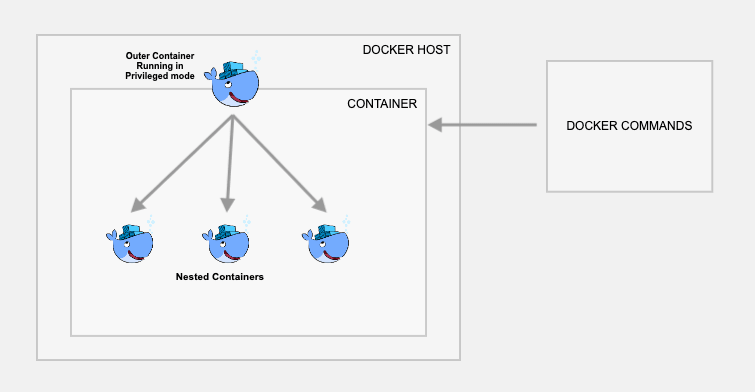
\includegraphics[width=.9\textwidth]{./images/docker-dind.png}
        \caption{DinD architecture.}
    \end{figure}
\end{frame}

\begin{frame}{Git LFS}
    \begin{figure}
        \centering
        \href{https://git-lfs.com/}{%
            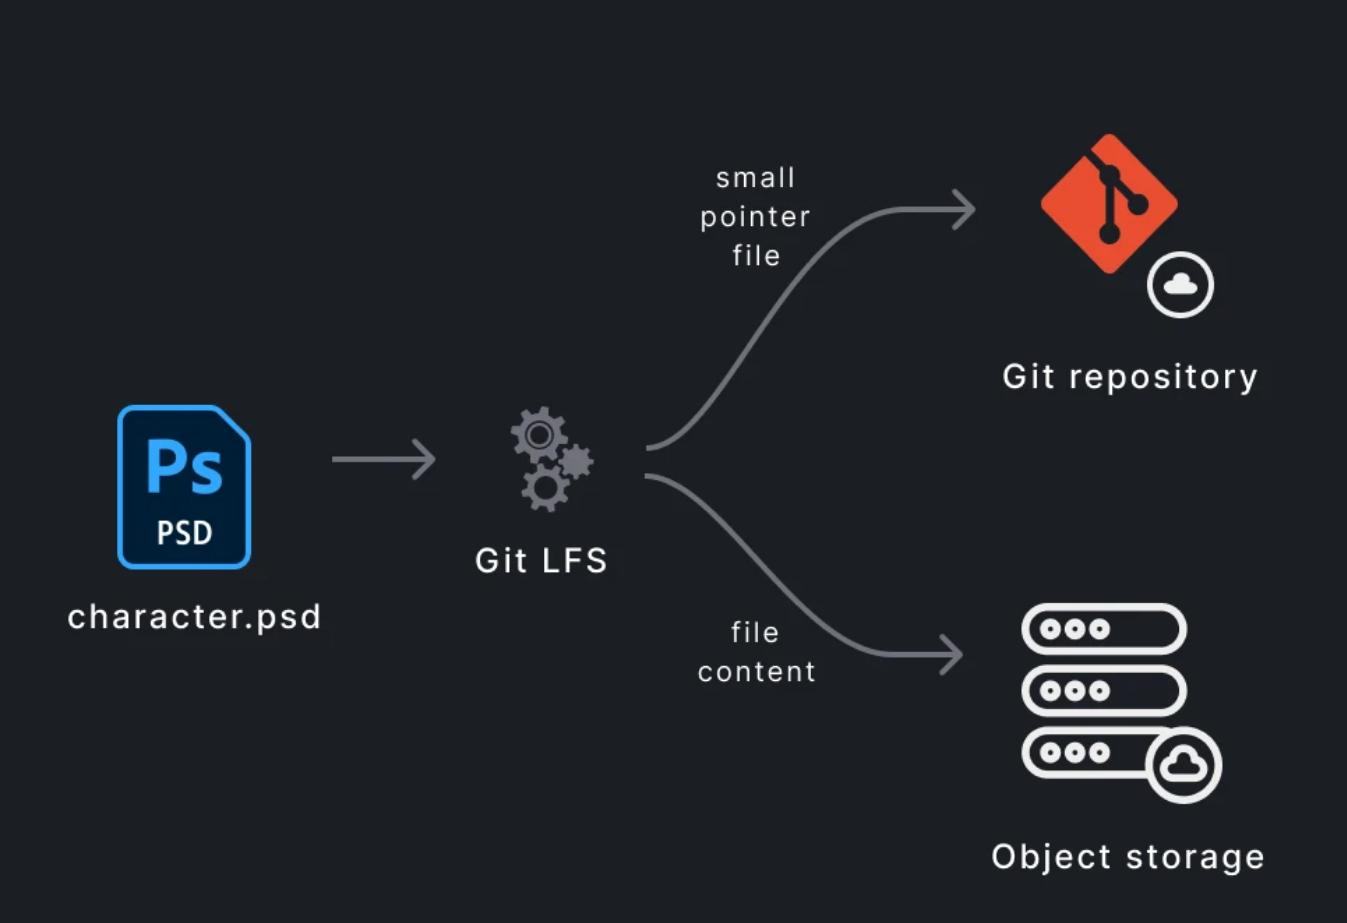
\includegraphics[width=.9\textwidth]{./images/Git-LFS.png}
        }
        \caption{Use Git LFS to track large files in your repository.}
    \end{figure}
\end{frame}

\begin{frame}{SagaLabs}
    \begin{figure}
        \centering
        \href{https://sagalabs.dk/}{%
            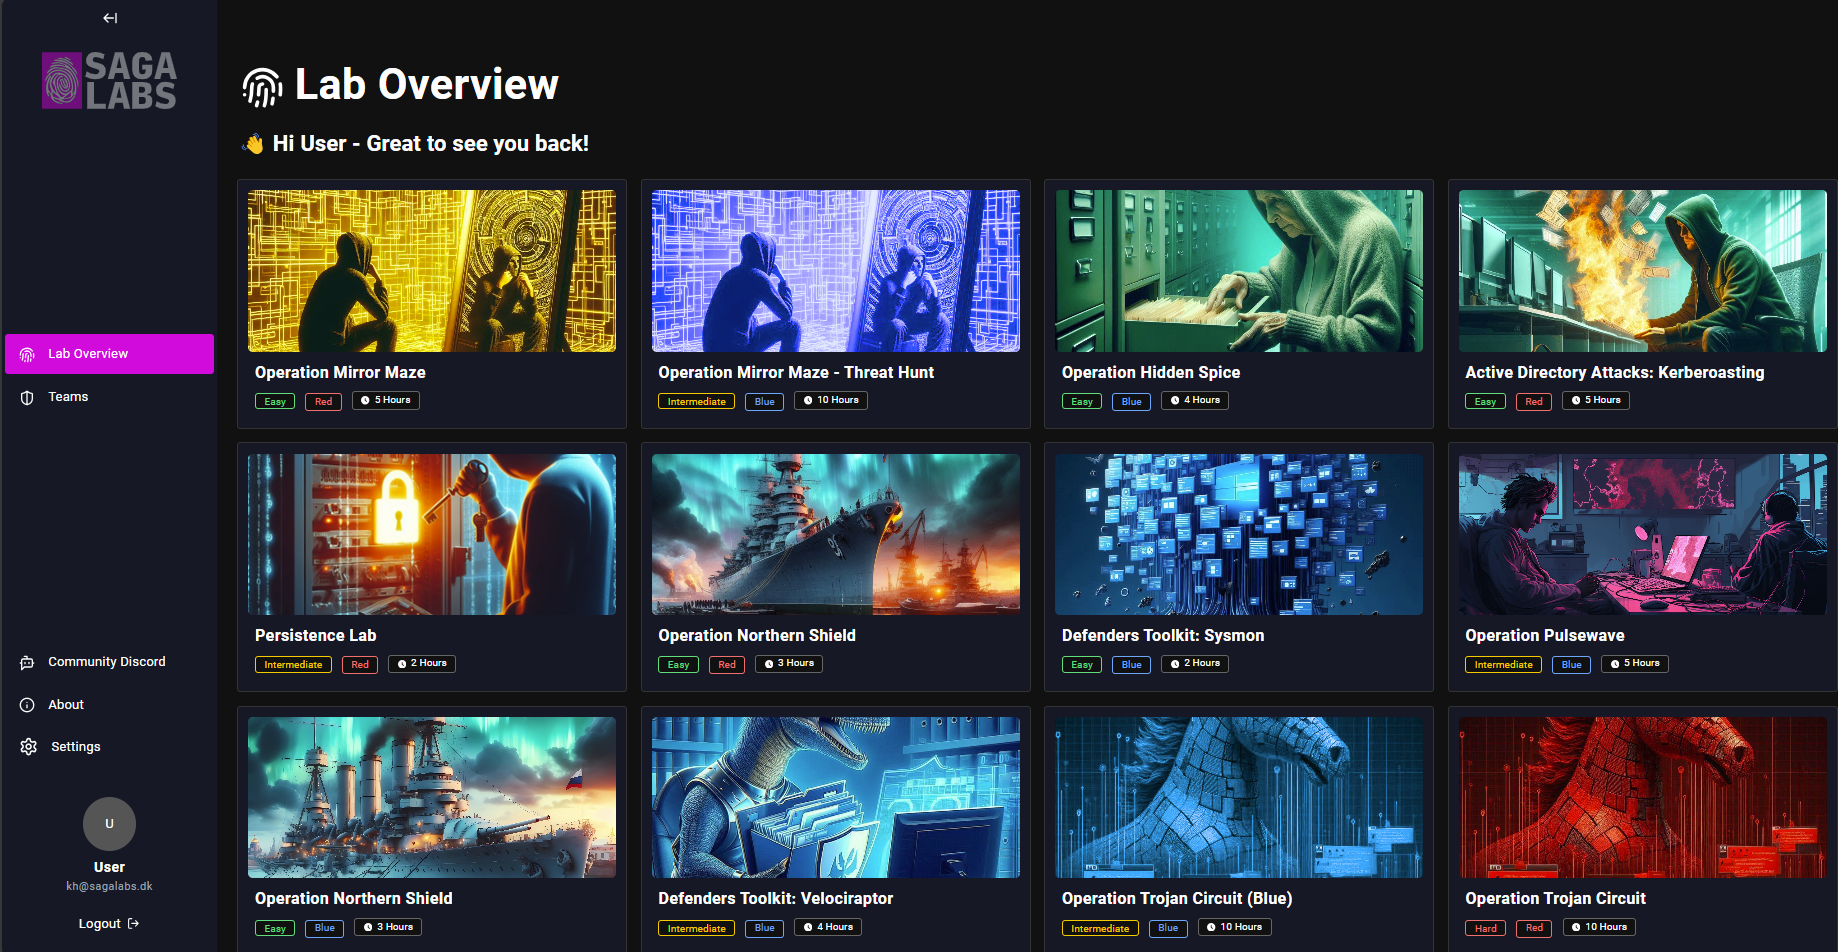
\includegraphics[width=1\textwidth]{./images/SagaLabs.png}
        }
        \caption{SagaLabs Platform.}
    \end{figure}
\end{frame}

\end{document}